% a line starting with "%" is a comment;
%that is, everything following "%" on the same line has no impact on the generated .pdf

%document on A4 sized paper with fontsize 12
\documentclass[12pt,a4paper]{article}

%font encoding (no need to pay attention to this)
\usepackage[T1]{fontenc}
\usepackage[utf8]{inputenc}

%packages for mathematical symbols and environments
\usepackage{amsmath,amssymb,amsthm}

%decent page margins
\usepackage{geometry}
\geometry{tmargin=2.5cm,bmargin=2.5cm,lmargin=2.5cm,rmargin=2.5cm}

%decent line spacing
\usepackage{setspace}
\onehalfspacing

% package that allows including grapics
\usepackage{graphicx}

%package for formatting urls 
\usepackage{url}

%the bibliography is done with natbib and uses the "Author (year)" style
\usepackage[authoryear]{natbib}

%avoids a faint print problem on some systems
\usepackage{ae,aecompl}

%define some mathematical environments
\newtheorem{lemma}{Lemma}
\newtheorem{proposition}{Proposition}
\newtheorem{example}{Example}
\newtheorem{assumption}{Assumption}
\newtheorem{result}{Result}
\newtheorem{theorem}{Theorem}
\newtheorem{corollary}{Corollary}
\newtheorem{definition}{Definition}

%%%%%%%%%%
%%%pretty formatting of (sub)section headings (no need to pay attention to this)
\makeatletter
\renewcommand{\section}{\@startsection{section}{1}{0mm}{-1.5\baselineskip}{0.8\baselineskip}{\normalfont\large\centering}}
\renewcommand{\subsection}{\@startsection{subsection}{2}{0mm}{-0.1\baselineskip}{0.5\baselineskip}{\normalfont\bf\flushleft}}
\renewcommand{\section}{\@startsection{section}{1}{0mm}{-0.9\baselineskip}{0.5\baselineskip}{\normalfont\large\centering}}
\renewcommand{\subsection}{\@startsection{subsection}{2}{0mm}{-0.1\baselineskip}{0.3\baselineskip}{\normalfont\bf\flushleft}}
\renewcommand{\@seccntformat}[1]{\csname the#1\endcsname
\hspace{+0mm}\large{.}\hspace{+1.9mm}}
\renewcommand{\@seccntformat}[2]{\csname the#1\endcsname
\hspace{+0mm}\large{.}\hspace{+1.9mm}}
\makeatother
%%%%%%%%%%%%


%%%%%%%%%%%%%%%%%%%%%%%%%%%%%%%%%%%%
%%%%%%% INSERT TITLE INFO HERE%%%%%%
%%%%%%%%%%%%%%%%%%%%%%%%%%%%%%%%%%%%
%allows to reference your title and name later on
\usepackage{titling}
%title of the thesis
\title{Your great thesis title}
%author
\author{Your Name}
% date: you can substitute "\today", which prints today's date, with some date of your choosing
\date{\today}
%%%%%%%%%%%%%%%%%%%%%%%%%%%%%%%%%%%%


%%% designing header and footer (if you prefer not to have a header and have page numbers at the bottome, just delete the following lines)
\usepackage{fancyhdr}
\pagestyle{fancy}
\fancyhead[L]{\theauthor} %left header is author name
\fancyhead[R]{\thetitle} %right header is thesis title
\fancyfoot[C]{\thepage} %center fotter is page number 

% if you want to remove the line separating header and text, remove the "%" on the next line
%\renewcommand{\headrulewidth}{0pt} 
%\renewcommand{\footrulewidth}{0pt}
%%%

%%%%%%%%%%%%%%%%%%%%%%%%%%%%%%%%%%%%%%%%%%%%%%
%%%%%%%%%%%%% DOCUMENT %%%%%%%%%%%%%%%%%%%%%%%
%%%%%%%%%%%%%%%%%%%%%%%%%%%%%%%%%%%%%%%%%%%%%%

\begin{document}

%%%%%%%% Title Page %%%%%%%%%%%%%%%%%%%%%%%%%
%% better leave the "titlepage" code alone unless you want to delete it altogether 
\begin{titlepage}
	\centering
	
\includegraphics[width=0.25\textwidth]{UoCseal}\par\vspace{1cm}
	{\scshape\LARGE University of Cologne \par}
	\vspace{1cm}
	{\scshape\Large Master Thesis in Economics\par}
	\vspace{1.5cm}
	{\huge\bfseries \thetitle \par}
	\vspace{2cm}
	{\Large\itshape \theauthor \par}
	\vfill
        \begin{tabular}{ccc}
          supervisor:&\hspace*{2cm}&second reader:\\
          Prof. Dr. \textsc{C. Schottmüller}&&\textsc{M. Gramb}
        \end{tabular}
	\vfill
        Submitted for Examination in the Study Programme \emph{Economics (M.Sc.)} \\at the \emph{Faculty of Management, Economics and Social Sciences}\\
        \vspace*{0.5cm}
% Bottom of the page
	{\large Cologne, \thedate\par}
\end{titlepage}
%%%%%%%%%%%%%%%%%%%%%%%%%%%%%%%%%%%%%%%%%%


%%%%%%%%%% Table of Contents etc. %%%%%%%%%
\pagenumbering{Roman}
\tableofcontents %creates table of contents
\newpage
\listoffigures %creates list of figures (delete this line if unnecessary)
\listoftables %creates list of tables (delete this line if unnecessary)
%%%%%%%%%%%%%%%%%%%%%%%%%%%%%%%%%%%%%%%%%%%

\newpage
%%%%%%Start of the actual content%%%%%%%%
\pagenumbering{arabic}
\section{Introduction}\label{sec:intro}

Here goes your introduction. This document can be used as a template (in this case you want to delete all my text from here to the \verb|\bibliographystyle{chicago}| comand) but I will also give some examples of how to cite and reference, and how to use mathematics in \LaTeX. Ideally, you should look at the .pdf and the .tex file at the same time to see what the code generates. 

\subsection{Literature Review}\label{sec:literature}

The literature review goes here. Let me give some examples how to cite in \LaTeX\ using BibTeX: I cite  \cite{stigler1980introduction} and \cite{jann2020informational} as examples (in the source file this reads \verb|\cite{stigler1980introduction}| where \verb|stigler1980introduction| is the label of this reference used in the .bib file.). A page in a book  is cited as \citet[p. 34]{solove2010privacy}. Note that all the cited articles, books etc. have to have an entry in the .bib file where you define the label used for citing and store all the information necessary for creating the reference list at the end of the document. You can usually copy and paste the entries for the .bib file from Google Scholar or JSTOR (and otherwise you do it by hand following Martin Osborne's guide). However, have a look at what you are copying and pasting as these automatic online references are sometimes incomplete.

The advantage of BibTeX is twofold: First, you spell the author names and the publication years correctly. Second, the reference list is automatically generated and formatted nicely.

Let me also comment on some common problems. First, how to cite a website? I suggest to cite websites as in \cite{LaTeXwiki} and articles on news websites or blogs as in \cite{nzzArt}. Second, capitalization in the reference list: The here chosen bibstyle will put all but the first letter of the title (of a journal article) in lower case. This should be avoided for names etc. To do so put capital letters in between curly brackets in the .bib file, e.g. ``On \{N\}ash equilibrium'' instead of ``On Nash equilbirium''. You can see an example for this in the BibTeX entry \cite{nzzArt}.

\section{Mathematics}\label{sec:math}

Mathematics within a line of text is put between \$ marks. For example, \verb|$\frac{3}{4}$| yields the fraction $\frac{3}{4}$ or $\lim_{x\rightarrow \infty}e^{-x}=0$ is generated by\\ % "\\" forces a linebreak; you should normally not use it
\verb|$\lim_{x\rightarrow \infty}e^{-x}=0$|. Subindeces as in $x_1$ are written as \verb|$x_1$|. Here is how you use math environments:

\begin{definition}[Fixed Point]\label{def:fp}
  Let $f: \,D\rightarrow R$ where $D,R\subseteq \mathbb{R}$. If $f(x)=x$, then $x$ is called a \emph{fixed point} of $f$.
\end{definition}

You reference the definition as ``definition \ref{def:fp}'' (that is \verb|definition \ref{def:fp}| in the source file where \verb|def:fp| is the label of the definition above). Similarly, you can reference sections as \verb|section \ref{sec:intro}| which yields ``section \ref{sec:intro}''. Also subsection \ref{sec:literature} can be referenced using \verb|subsection \ref{sec:literature}|. The advantage of such references over writing ``section 1.1'' directly is that your references will automatically adjust if you change something in the structure of your document; for example, if you insert another section.
(Note that you have to compile \LaTeX\ twice before it gets a new reference properly formatted.)

Note that you can generate numbered equations that can be similarly referenced as follows:
\begin{equation}
  \label{eq:fixedPoint}
  f(x)=x.
\end{equation}
This equation can be referenced as equation (\ref{eq:fixedPoint}), i.e. \verb|(\ref{eq:fixedPoint})| in the source file where \verb|eq:fixedPoint| is the label of the equation above.

To get several equations in a row with aligned equality signs you can use the align environment where \verb|&| indicates the position that should be aligned and \verb|\\| indicates a linebreak, i.e. the start of the next equation:

\begin{align}
  f(x)&=x \label{eq:f} \\
  g(x)&=x^2+x+5     \label{eq:g}
\end{align}

Each equation can be referenced on its own like equation (\ref{eq:f}) or equation (\ref{eq:g}) here.

\section{Results}\label{sec:results}


A mathematical result, like a proposition, is written in a similar environment as a definition.

\begin{proposition}\label{prop:fp01}
  Let $f: \,[0,1]\rightarrow[0,1]$ be an increasing function. Then, $f$ has a fixed point.
\end{proposition}

\section{Font face and miscellaneous formatting}
\label{sec:formatting}

If you want to \emph{emphasize} a certain word or part of a sentence, you do so using the command \verb|\emph{whatever you want to emphasize}|. You can also use \textbf{bold fonts} using the command \verb|\textbf{whatever should be in bold}|. 
\par
Another useful hint concerns paragraph formatting. If you want to start a new paragraph, you either have to leave a blank line in your code (hit Enter twice) or you use the command \verb|\par|. A normal linebreak occurs if you use \verb|\\| but please do not use this to start a new paragraph as it does not indent the first line of the next paragraph which is considered bad style. (I do it here nevertheless, so you see the difference.)\\
At some point you may want to use an enumeration. \LaTeX provides the enumerate environment for this:
\begin{enumerate}
  \item first item
  \item second item
  \item third item.
\end{enumerate}

You can even have subenumerations inside an enumeration:
\begin{enumerate}
  \item first item
  \item second item with following subitems
    \begin{enumerate}
      \item subitem one
      \item subitem two
    \end{enumerate}
  \item third item
\end{enumerate}

For lists that are not numbered, there is  the itemize envrionment:
\begin{itemize}
  \item first item
  \item second item
  \item third item.
\end{itemize}

\section{Figures and Tables}\label{sec:ext}

You can include a graphic with the command \verb|\includegraphics{filename}| (recommended file formats are png, eps or pdf). Usually, it is a good idea to place the graphic in a figure environment as here:

\begin{figure}[h]
  \centering
  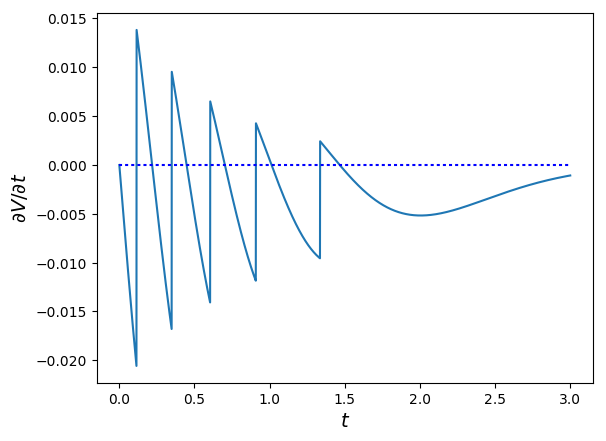
\includegraphics[scale=0.6]{Vprime} %the scale parameter adjusts the size of the figure (to check, try out 1 instead of 0.6 and compile) 
  \caption{A nice figure}
  \label{fig:zigzag}
\end{figure}

We can reference the figure as figure \ref{fig:zigzag} using its label.

Sometimes you need to have a nicely formatted table. I give a simple example; see \url{https://en.wikibooks.org/wiki/LaTeX/Tables} for more on this. In case you want to present a regression output in a table, please note that there are packages producing \LaTeX tables for the most common statistics programmes.

\begin{center}
  \begin{table}[h]
    \centering
    \begin{tabular}{|l|l|c|l|} \hline
  Country &Capital  & Population    & Source \\ \hline
  China   & Beijing & 1,404,556,640 & National population clock\\
  Japan   & Tokio   & 125,930,000   & Monthly provisional estimate \\
  Germany & Berlin  & 83,157,201    & National quarterly estimate\\ \hline
\end{tabular}
\caption{Countries and their population}
\label{tab:pop}
\end{table}
\end{center}

\begin{center}
  \begin{table}[h]
    \centering
    \begin{tabular}{l|l|c|l} 
  Country &Capital  & Population    & Source \\ \hline
  China   & Beijing & 1,404,556,640 & National population clock\\
  Japan   & Tokio   & 125,930,000   & Monthly provisional estimate \\
  Germany & Berlin  & 83,157,201    & National quarterly estimate
\end{tabular}
\caption{Countries and their population a bit simpler}
\label{tab:pop}
\end{table}
\end{center}

\section{Conclusion}

All scientific writing should be done in \LaTeX.

%start what follows on a new page
\newpage

%after this command new sections will be labeled alphabetically
\appendix

\begin{center}
  \begin{Large}
Appendix
\end{Large}
\end{center}

\section{Proofs}\label{sec:proofs}
\noindent\textbf{Proof of proposition \ref{prop:fp01}:} Let 
\begin{equation} \label{eq:A}
A=\{x:\;x\leq f(x)\}.
\end{equation}
As $f$ maps into $[0,1]$, $0\leq f(0)\in[0,1]$ and therefore $0\in A$ and $A\neq\emptyset$. Let $x^*=\sup A$.

 $f(x^*)\leq x^*$: suppose not, i.e. suppose $f(x^*)>x^*$, let $\varepsilon =f(x^*)-x^*>0$ and observe that $x^*+\varepsilon <f(x^*)  \leq f(x^*+\varepsilon )$ because $f$ is increasing. Hence, $x^*+\varepsilon \in A$ which contradicts the definition of $x^*$.

$f(x^*)\geq x^*$:  if $x^*\in A$, this holds by the the definition of $A$, see equation (\ref{eq:A}). But $x^*\in A$ has to hold by the definition of $x^*$ as otherwise $f$ would have to discontinously drop downward at $x^*$ contradicting that $f$ is increasing.

Hence, $x^*=f(x^*)$. \qed
 
\section{Second Appendix}\label{sec:otherAppendix}

Another section in the appendix.

%start what follows on a new page
\newpage

%style of the bibliography
\bibliographystyle{chicago}
%name of the .bib, here "privacy.bib", file that has to be in the same folder as this .tex file
\bibliography{privacy}


\end{document}